\chapter{Ligand binding sites prediction} \label{ch:2}

Great progress has been made in the field of the ligand binding sites prediction within the last 20 years. The existence of various projects and experiments, such as CASP (Critical Assessment of protein Structure Prediction) \cite{casp_def}, CAMEO (Continuous Automated Model EvaluatiOn) \cite{cameo} or CAFA (Critical Assessment of Function Annotation) \cite{cafa}, motivates the development of this field and provides standardized evaluation measures \cite{methods}. Plethora of tools based on different approaches has been developed, from simple geometry based algorithms to recently emerging deep learning based methods. Zhao \textit{et al.} \cite{methods} published a review summarizing and categorizing more than 50 different methods.

The tools can vary in many aspects. Some of them are stand-alone command line tools running in fully automated manner, other are available as web-servers only, providing interactive interface. Some tools require some kind of pre-processing or supplying pre-calculated files, e.g. sequence alignments. The tools can differ in speed of prediction. In a survey comparing the running times of several methods published by Krivák and Hoksza \cite{p2rank1}, the differences of times required for prediction on a single protein were in order of magnitude. FPocket \cite{fpocket}, the fastest of compared tools, can return prediction for one protein in 0.2 s, while getting prediction from the COACH web-server \cite{coach} would take 15 hours. The choice of a suitable tool depends on a use case: for processing large datasets, a fully automated and fast tool is required, whereas for inspecting several structures manually, when the speed is not the priority, a slower but more accurate method can be used.

In this Chapter, we summarize different strategies with specific examples of existing methods, we present P2Rank method in more detail and we explain how the performance of the predictors can be evaluated.

\section{Existing methods}

The existing methods for the protein-ligand binding sites prediction are based on various strategies and algorithmic approaches. It is possible to classify them into following caterogies; neverthless, keep in mind that many tools use a combination of the following approaches.

\subsection{Geometry based approach}
Most small ligands bind to concave cavities and pockets on the protein surface, as was observed in many studies of protein-ligand complexes in PDB \cite{methods}. The geometric methods make use of this information and employ various techniques for calculating certain geometric measures from the protein structure. Some methods use additional properties such as polarity or charge, for instance FPocket \cite{fpocket} which calculates properties from the atoms in order to score each pocket. Other are purely geometrical, such as PocketPicker \cite{pocketpicker}, a grid-based technique that uses a buriedness index to identify clusters of grid points where a ligand is likely to bind.

\subsection{Energy based approach}
Energy based methods predict the binding sites by calculating interaction energies between residues on the protein surface and a probe (for example methyl group in case of Q-SiteFinder \cite{qsitefinder}). The probe is placed on the grid points around the whole protein's surface and energetically most favourable locus is selected as putative binding site.

\subsection{Evolutionary approach}
These methods make use of conservation scores computed for each residue from the protein primary sequence. The conservation can be used to rescore the predicted sites (LIGSITE\textsuperscript{CSC} \cite{ligsite}) or it can be used directly for the prediction (ConCavity \cite{concavity}).

\subsection{Template based approach}
The template based methods make use of the fact that homologous proteins share similar folds and can bind ligands at similar positions. These methods rely on databases of protein-ligand complexes and use these complexes as templates to derive the predictions. Template based methods usually yield high confidence predictions; however, they are not able to discover novel binding sites \cite{p2rank1}. There are two main types: structure template based methods (e.g. FINDSITE \cite{findsite} which uses threading (fold recognition) algorithm) and sequence template based methods (e.g. S-SITE \cite{coach}, using Needleman-Wunsch dynamic programming algorithm \cite{needleman}).

\subsection{Machine learning approach}
Predicting protein-ligand binding sites can be seen as a classification problem. Many algorithm have been employed, for instance Suport Vector Machines (eFindSite \cite{efindsite}), Random Forests (P2Rank \cite{p2rank1}), K-means clustering (ConCavity \cite{concavity}), multiple linear regression (SFCscore \cite{sfcscore}) or artificial neural network (NNScore \cite{nnscore}). In the recent years, deep learning based prediction methods became popular in the field. Most of the methods use convolutional neural networks (CNN), e.g. DeepSite \cite{deepsite} or DeepCSeqSite \cite{deepcseqsite}.

\subsection{Consensus approach}
The consensus methods combine results of other existing methods and by this approach, they can achieve better results than the individual methods. For instance, MetaPocket 2.0 \cite{metapocket} combines eight different methods, taking top three sites from each of them. The resulting 24 sites, which can be spatially overlapping, are merged together by hierarchical clustering.


\section{Evaluation of success rates}

According to the way they represent prediction results, there are two types of predictors: \textit{residue-centric} and \textit{pocket-centric}. The residue-centric methods see the problem of binding sites prediction as binary classification. Each residue on the surface is classified as binding or non-binding. On the other hand, the pocket-centric methods do not classify individual residues; rather, they output a list of putative binding sites, usually represented as pocket centers, or sets of points around the protein surface, representing the shape of the binding site. The output list usually contains more predicted sites than the number of ligands and therefore, there are many false positives. Most methods rank the output list by the probability of being a true binding site, obtained by various ranking algorithms \cite{p2rank1}. Ranking is important to prioritize the results, e.g. for visual inspection.

Residue-centric methods can be evaluated and compared by standard performance measures of binary classificators, such as accuracy, precision, recall, MCC (Matthews Correlation Coefficient) or AUC (Area Under the Curve) \cite{classification}.

To evaluate the performance of pocket-centric ligand binding sites predictors, Chen \textit{et al.} \cite{benchmark} proposed evaluation methodology with ligand-centric approach. The problem with previous protein-centric approach arises when a protein has more than one ligand. That approach requires only one correctly predicted binding site per protein to achieve 100\% success rate, regardless of the number of ligands.

In the ligand-centric approach, to achieve 100\% success rate we want a method to correctly identify binding sites for all ligands in the dataset. Every ligand is equally relevant for the final success rate. The output of a method is a ranked list of putative sites. The list usually contains more sites than the number of ligands and therefore, many of them are false positives. For this reason, we take only the top-ranking sites into consideration for the evaluation. If all the predicted sites were considered, the most successful method would be the one returning so many binding sites they would cover the whole protein surface, which is certainly not desirable. The cutoffs Top-\textit{n} and Top-(\textit{n}+2) were used for the evaluation of P2Rank \cite{p2rank1} (\textit{n} is the number of ligands). A binding site is considered correctly identified if at least one of the Top-\textit{n} or Top-(\textit{n}+2) binding sites passes a detection criterion (defined below). The success rate is then the number of correctly predicted sites divided by the total number of sites.

The position or shape of a predicted binding site does not have to match the true binding site precisely. Chen \textit{et al.} \cite{benchmark} described several detection criteria to decide when the prediction is correct:

\begin{itemize}
\item $D_{CA}$ - a binding site is correctly predicted if the minimal distance between the center of the predicted site and any atom of the ligand is not greater than an arbitrary threshold D. The threshold D is usually 4 {\AA}.
\item $D_{CC}$ - a binding site is correctly predicted if the minimal distance between the center of the predicted site and the centrer of the ligand is not greater than D. This measure compensates for the size of the ligand (unlike $D_{CA}$, it does not give higher success rates to larger ligands).
\item $O_{PL}$ - this measure expresses normalized spacial overlap between the predicted binding site and the ligand. It is defined as the volume of the intersection of the predicted site and the ligand, divided by the union of the two volumes. It is the most precise of the three measures, as it takes into account the spacial orientation. The disadvantage is that it can be computed only for the methods outputing the full set of grid points representing the site, instead of simply reporting the center of the site.
\end{itemize}

The first two criteria were used to evaluate the success rate of P2Rank method.

\section{P2Rank}

P2Rank \cite{p2rank1} is a machine learning based ligand binding sites predictor developed by Radoslav Krivák and David Hoksza at Charles University. It is an open-source tool available as a stand-alone command line program or a web-server \cite{prankweb}. The command line tool is platform-independent, it is implemented in Java and Groovy and is very lightweight, as it does not depend on large structural or sequence databases, or any other bioinformatics tools. It is especially suitable for large datasets, thanks to its speed which can be less than 1 s per protein. 

P2Rank uses Random Forests classifier \cite{randomforests} to predict ligandability of specific regularly spaced points (\textit{SAS points}, as described below) located around the surface of the protein, according to properties of their local neighborhoods. Random Forests is an ensemble learning method, combining a multitude of decision trees created by taking bootstrap samples from the training dataset and randomly selecting features for individual trees training.

The method takes a list of PDB files as input, and for each structure, outputs a ranked list of predicted binding sites. For each structure, the predictions are obtained following these steps: \cite{p2rank1, p2rank2}

\begin{enumerate}
\item Calculate protein's solvent-accessible surface \cite{shrake} and generate a set of equally spaced points (called \textit{SAS points}) along this surface. Each point will represent its local neighborhood. The default spacing is approximately 1.5 {\AA}. 
\item For each SAS point, calculate a feature vector based on its local chemical neighborhood. Some features are calculated directly on the SAS point (e.g. \textit{protrusion}, a measure of point's `buriedness'); other are projected from the nearby protein atoms, weighted by their distance. The features can be defined on the atomic level (e.g. B factor), or residue level (e.g. hydrophobicity). Altogether, the vector consists of 35 features.
\item The Random Forests classifier predicts ligandability scores for each SAS point, based on its feature vector. Instead of working with binary output (ligandable/nonligandable), the score ranges from 0 to 1 (1 = ligandable).
\item Filter out the SAS points with ligandability scores below certain threshold. Then apply single linkage clustering with 3 {\AA} cutoff on the rest. Resulting clusters represent predicted binding sites. Only clusters with 3 or more points are considered.
\item Rank predicted binding sites to place the most promising ones to the top. The ranking score is defined as the sum of squared ligandability scores of all SAS points defining the site.
\end{enumerate}

\begin{figure}[!h]\centering
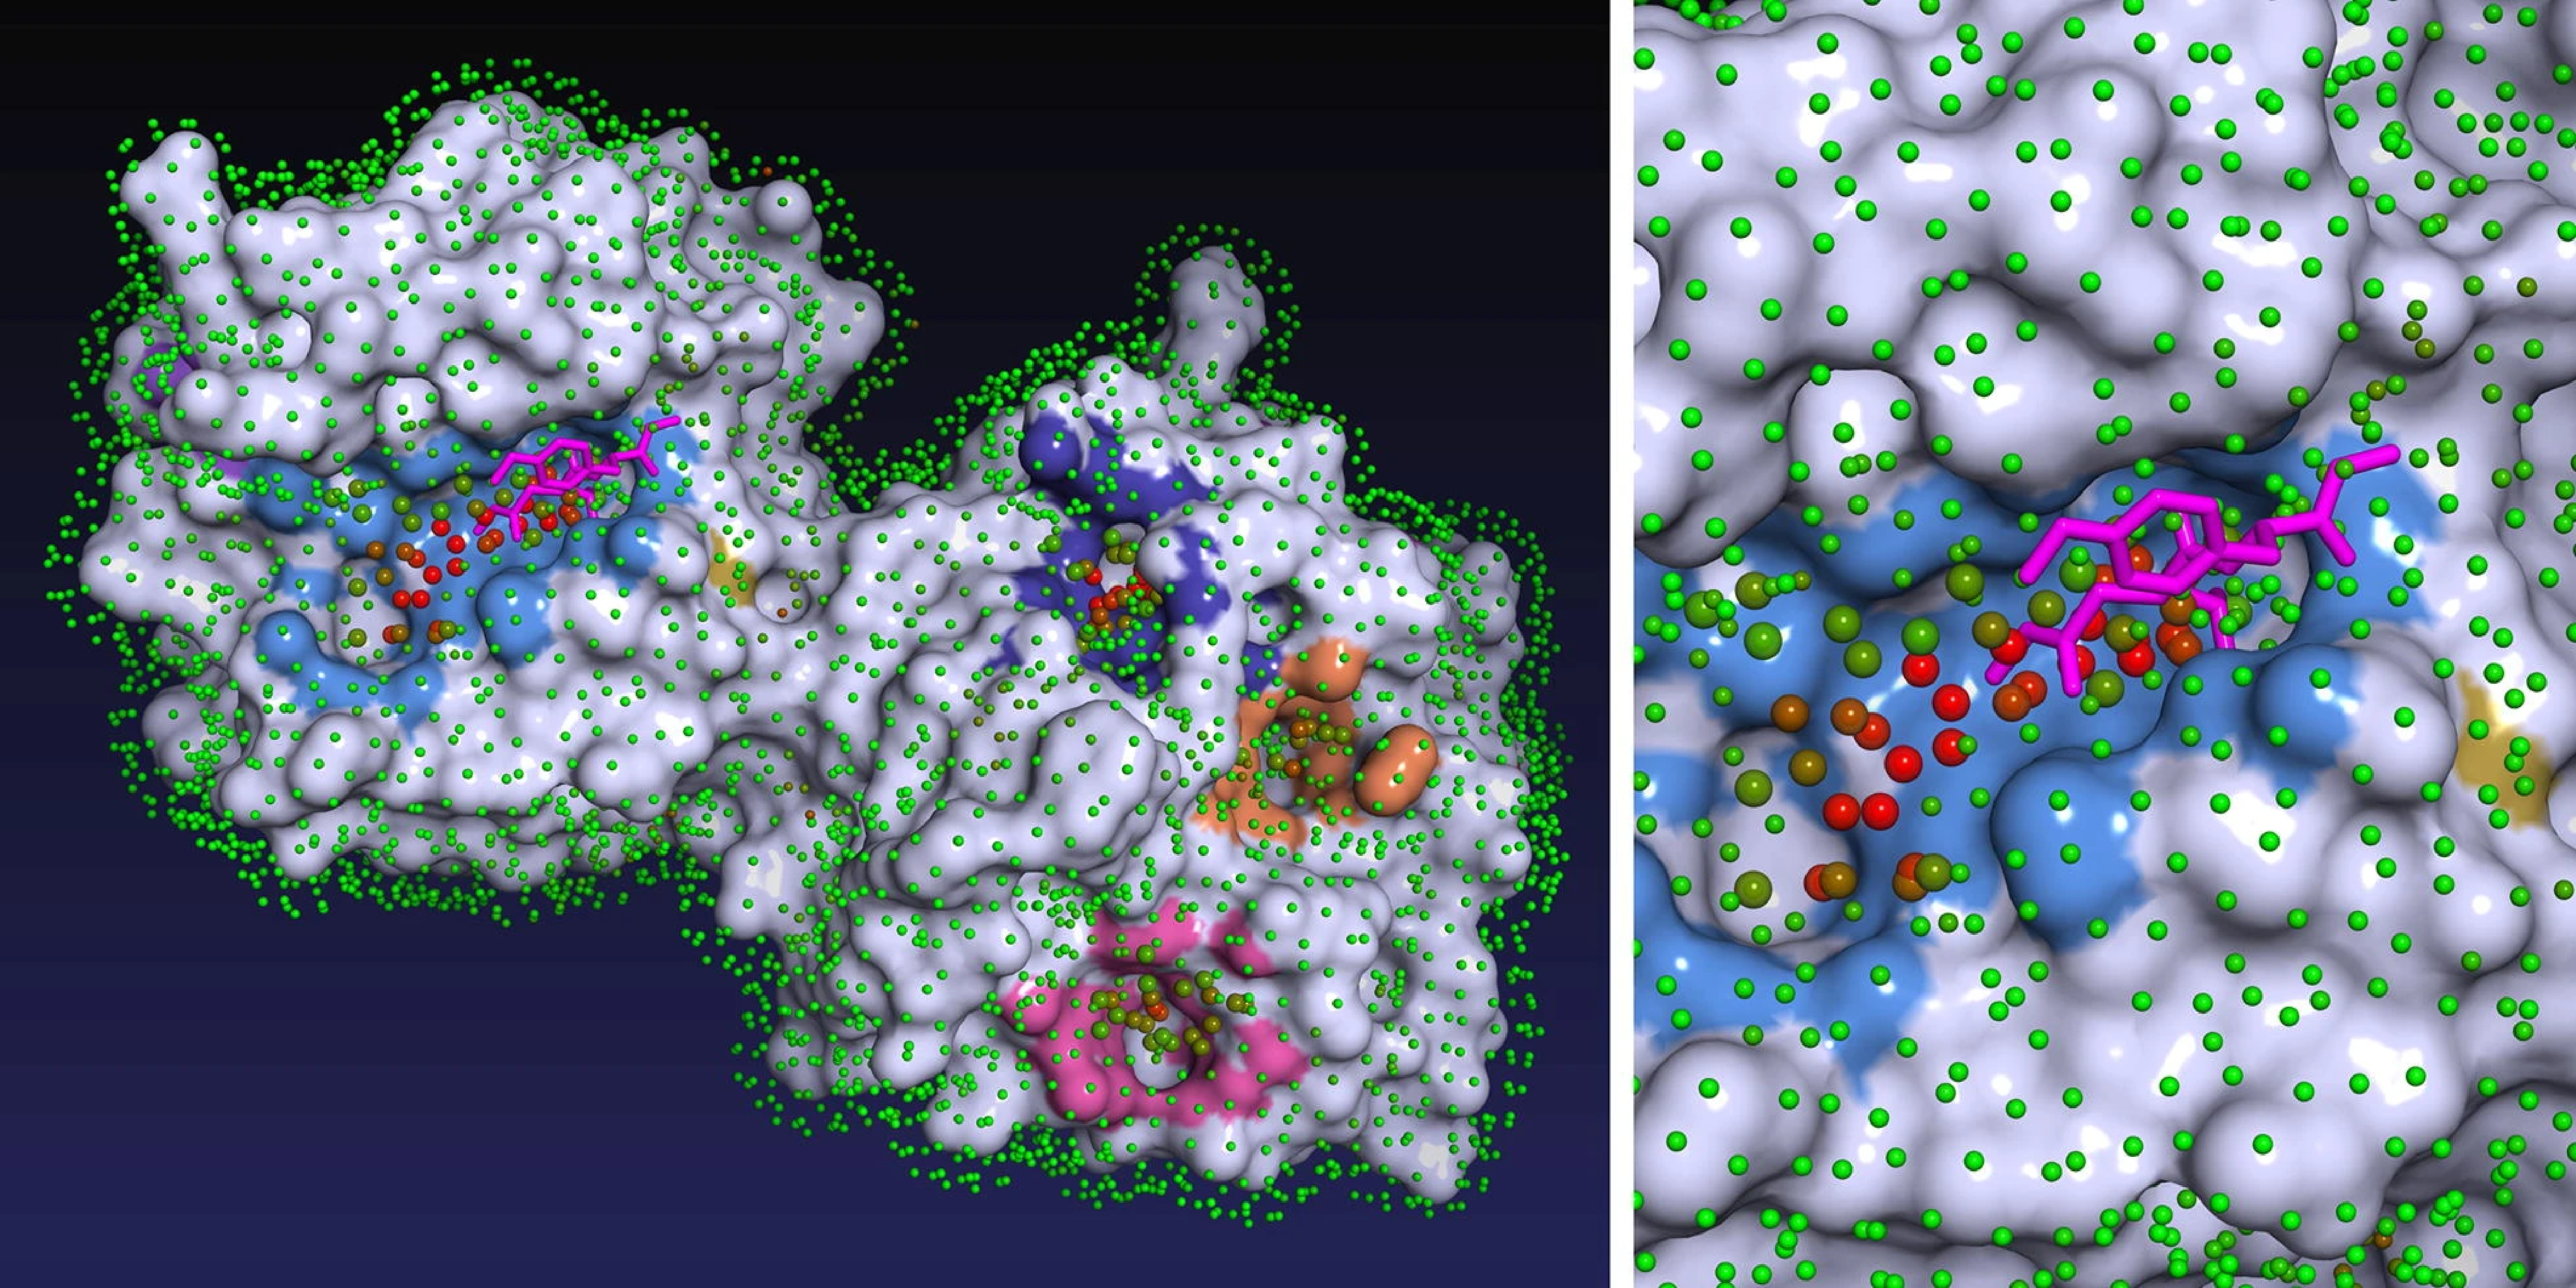
\includegraphics[width=145mm]{../img/p2rank.pdf}
\caption{Visualization of SAS points for structure 1FBL. Each point is colored by its predited ligandability score (red points are the most ligandable, green points the least). Predicted binding sites are marked by coloured protein surface. Adapted from: \textit{P2Rank: machine learning based tool for rapid and accurate prediction of ligand binding sites from protein structure} \cite{p2rank1}}
\label{fig:p2rank}
\end{figure}

Figure~\ref{fig:p2rank} illustrates computed SAS points and predicted binding sites on an example structure.

In theory, any classifier could be used in step 3. Random Forests algorithm was chosen for several reasons. First of all, it has great generalization ability. Random Forests are great when dealing with highly correlated variables \cite{forests_biology} which is a very useful property for this application, as the feature vector contains a lot of related variables (e.g. various amino acid properties, such as hydrophobicity, polarity, aromaticity, charge etc.). It can cope with a large number of irrelevant variables, as well as binary and ordinal variables. Furthermore, it is relatively robust to outliers and noise, easily parallelized and simple to use, as it does not require prior scaling or other transformations of features. Also, it is faster than many other classifiers. And finally, it is able to report internal estimates of individual variable importances, which can give valuable insight into the problem \cite{randomforests, forests_biology, p2rank2}.

P2Rank comes with a pre-trained optimized default model trained on Chen11 dataset \cite{benchmark}, built with 100 trees, each grown with no depth limit using 6 features. In addition, a user can train and evaluate new models on his or her own datasets. This can be very useful for creating models specialized on certain types of proteins or ligands. The latest version of P2Rank also allows to add a custom feature to the feature vector without changing P2Rank source code. This possibility was employed for the experiments in this thesis. The feature values are supplied in CSV files (one file per structure) where one row describes one residue (or atom).

More details on setup, requirements, usage examples, models training and evaluation and adding new features can be found in the project's repository (\url{https://github.com/rdk/p2rank}) or in the tutorial available at \url{https://github.com/cusbg/p2rank-framework}.


